\documentclass[fleqn]{jsarticle}

\usepackage{graphicx}
\usepackage{amsmath,amssymb}
\usepackage{amsmath}
\usepackage{fancyhdr}

\pagestyle{fancy}
\fancyhead[RE,RO]{先端データ解析論 レポート}

\usepackage{xcolor}
\usepackage[justification=centering]{caption}
\usepackage{listings}
\renewcommand{\lstlistingname}{リスト}
\lstset{language=Python,%
        % basicstyle=\footnotesize,%
        basicstyle=\tiny,%
        commentstyle=\textit,%
        classoffset=1,%
        keywordstyle=\bfseries,%
      	frame=tRBl,framesep=5pt,%
      	showstringspaces=false,%
        linewidth=35em,
      	}%

\begin{document}

\newcommand{\argmax}{\mathop{\rm argmax}\limits}
\newcommand{\argmin}{\mathop{\rm argmin}\limits}

\title{先端データ解析論 第3回レポート}
\author{電子情報学専攻 48-176403 石毛真修}
\maketitle



\section*{大問1.}
線形モデル $f_\theta(\mathbf x) = \sum^b_{j=1} \theta_j \phi_j(\mathbf x)$
に対する重み付き最小二乗法
\begin{eqnarray*}
  \hat{\theta} = \argmin_\theta \frac{1}{2} \sum^n_{i=1} \tilde{\omega_i} \left(f_\theta(\mathbf x)_i - y_i\right)^2
  = (\Phi^{\mathrm T} \tilde{W} \Phi)^-1 \Phi^{\mathrm T} \tilde{W} \mathbf{y}
\end{eqnarray*}

\subsubsection*{証明}
\begin{eqnarray*}
  \Phi = \begin{bmatrix}
    \phi_1({\mathbf x}_1) &\phi_2({\mathbf x}_1) &... &\phi_b({\mathbf x}_1)\\
    \phi_1({\mathbf x}_2) &\phi_2({\mathbf x}_2) &... &\phi_b({\mathbf x}_2)\\
    ...\\
    \phi_1({\mathbf x}_n) &\phi_2({\mathbf x}_n) &... &\phi_b({\mathbf x}_n)\\
  \end{bmatrix}
\end{eqnarray*}


とする。


誤差関数 $\frac{1}{2} \sum^n_{i=1} \tilde{\omega_i} \left(f_\theta(\mathbf x)_i - y_i\right)^2$ を$J$とおくと

\begin{eqnarray*}
  J &=& \frac{1}{2} (\hat{\mathbf y} - \mathbf y)^{\mathrm T} \tilde W (\hat{\mathbf y} - \mathbf y)\\
  &=& \frac{1}{2} (\Phi \mathbf \theta - \mathbf y)^{\mathrm T} \tilde W (\Phi \mathbf \theta - \mathbf y)\\
  &=& \frac{1}{2} \left[ \mathbf{\theta}^\mathrm{T} \Phi^\mathrm{T} \tilde W \Phi \mathbf \theta
    - \mathbf{\theta}^\mathrm{T} \Phi^\mathrm{T} \tilde W \mathbf y - \mathbf{y}^{\mathrm T} \tilde W \Phi \mathbf \theta
    + \mathbf{y}^{\mathrm T} \tilde W \mathbf y \right]
\end{eqnarray*}


この$J$ を最小化したいので、$\frac{dJ}{d\mathbf \theta} = 0$ とすると、
\begin{eqnarray*}
  \frac{dJ}{d\mathbf \theta} &=& \frac{1}{2} \left[ 2 \Phi^{\mathrm T} \tilde W \Phi \mathbf \theta
    - \Phi^{\mathrm T} \tilde {W} \mathbf y - (y^{\mathrm T} \tilde W \Phi)^{\mathrm T} \right]\\
  &=& \frac{1}{2} \left[ 2 \Phi^{\mathrm T} \tilde W \Phi \mathbf \theta - 2 \Phi^{\mathrm T} \tilde {W} \mathbf y \right]\\
  &=& \Phi^{\mathrm T} \tilde W \Phi \mathbf \theta - \Phi^{\mathrm T} \tilde {W} \mathbf y
\end{eqnarray*}
\begin{eqnarray*}
  \therefore \hat{\mathbf \theta} = (\Phi^{\mathrm T} \tilde{W} \Phi)^-1 \Phi^{\mathrm T} \tilde{W} \mathbf{y}
\end{eqnarray*}





\section*{大問2.}
微分可能で対称な損失関数$\rho(r)$ に対して$\tilde{r}$ で接する二次上界は、
\begin{eqnarray*}
  \tilde{\rho}(r) = \frac{\tilde{\omega}}{2} r^2 + const
\end{eqnarray*}

\subsubsection*{証明}
$\rho(r)$ は対称なので、それに接する二次上界$\tilde{\rho}(r)$ も対称になる。よって、
\begin{eqnarray*}
  \tilde{\rho}(r) = a r^2 + b
\end{eqnarray*}


接しているという条件から、接点の傾きが同じであり、かつ共通の解を持つので、
\begin{eqnarray*}
  \rho'(\tilde r) &=& 2 a \tilde{r}\\
  \rho(\tilde r) &=& a \tilde{r}^2 + b
\end{eqnarray*}

これを解いて、
\begin{eqnarray*}
  a = \frac{1}{2} \frac{\rho'(\tilde r)}{\tilde r} \hspace{2em} b = \rho(\tilde r) - \frac{1}{2} \rho'(\tilde r) \tilde r
\end{eqnarray*}

よって、
\begin{eqnarray*}
  \tilde{\rho}(r) &=& \frac{1}{2} \frac{\rho'(\tilde r)}{\tilde r} r^2
    + \left( \rho(\tilde r) - \frac{1}{2} \rho'(\tilde r) \tilde r \right)
  = \frac{\tilde \omega}{2} r^2 + const
\end{eqnarray*}

\newpage
\section*{大問3.}
まず、次のようなデータ直線$y=x$ に正規分布から生成されるノイズを載せたデータを作成する。
\begin{center}
\begin{tabular}{c}
  \begin{lstlisting}[]
    import matplotlib
    import matplotlib.pyplot as plt
    import numpy as np

    n, N = 10, 1000
    x = np.linspace(-3, 3, n)
    X = np.linspace(-4, 4, N)

    # Original data
    np.random.seed(5)
    y = x + 0.2 * np.random.normal(size=n)
    y[2], y[n -2], y[n - 1] = [-4] * 3
  \end{lstlisting}
\end{tabular}{c}
\end{center}


次に、適当に初期化したパラメータthetas = [theta1, theta2] を元に、繰り返し最小二乗法を行うことで
Tukey回帰を行う。なお、コード中の変数Phiは計画行列である。
\begin{center}
  \begin{tabular}{c}
    \begin{lstlisting}[]
      # Tukey Regression
      Phi = np.array([[1, x[i]] for i in range(n)])
      thetas = np.random.normal(1, 0.1, 2)
      ETA = 2
      def w_tukey(r):
          return (1 - (r**2)/(ETA**2))**2 if np.absolute(r) <= ETA else 0
      # Iteration
      for step in range(20):
          errors = y - np.matmul(Phi, thetas)
          _W = np.diag([w_tukey(err) for err in errors])
          Q = Phi.T @ _W @ Phi
          if np.linalg.det(Q) == 0:
              break
          thetas = np.linalg.inv(Q) @ Phi.T @ _W @ y
    \end{lstlisting}
  \end{tabular}{c}
\end{center}

最後にこれをプロットする。
\begin{center}
  \begin{tabular}{c}
    \begin{lstlisting}[]
      # Prediction
      def pred(x):
          return thetas[0] + thetas[1] * x

      plt.scatter(x, y)
      plt.plot(X, pred(X), 'b-')
      axes = plt.gca()
      axes.set_ylim([-4.5, 3])
      plt.show()
    \end{lstlisting}
  \end{tabular}{c}
\end{center}


\begin{figure}[h]
  \begin{center}
    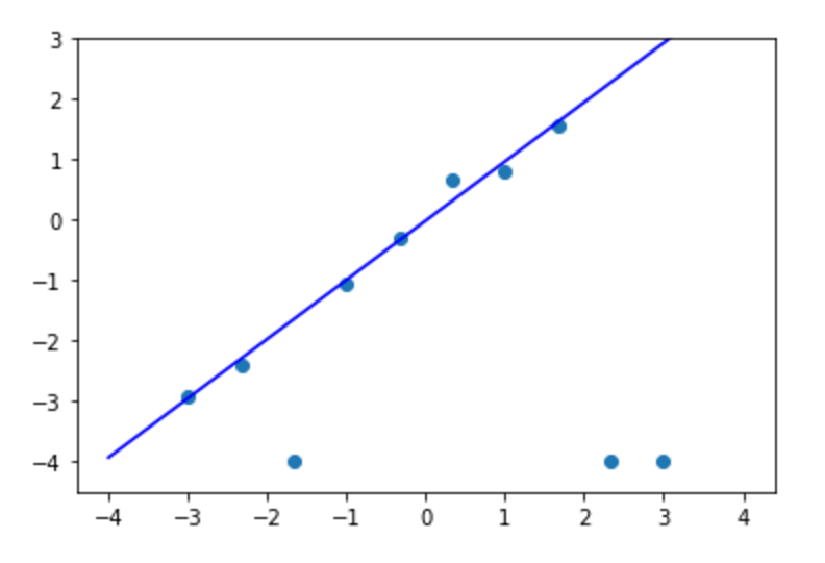
\includegraphics[width=0.6\textwidth]{figs/TukeyRegression.eps}
  \end{center}
  \caption{Tukey回帰の結果}
\end{figure}


\end{document}
